% $Header$

\documentclass{beamer}



\usetheme{metropolis}
\usepackage[english]{babel}
\usepackage[T1]{fontenc}
\usepackage{graphicx}
\usepackage{caption} %To use \caption*


\usepackage{listings}
\usepackage{xcolor}

\lstset{
    language=R,                     % set language
    basicstyle=\ttfamily\small,     % font style
    numbers=none,
    %numbers=left,                   % line numbers on the left
    numberstyle=\tiny,              % line number style
    stepnumber=1,                   % number every line
    numbersep=5pt,                  % space between numbers and code
    backgroundcolor=\color{gray!10},% light gray background
    keywordstyle=\color{blue},      % keywords in blue
    commentstyle=\color{green!50!black}, % comments in green
    stringstyle=\color{red},        % strings in red
    breaklines=true,                % allow line breaking
    frame=single,                   % border around code
    tabsize=4                       % tab size
}% 1. DEFINE THE LOGO HERE (Preamble)
% We use \hspace* to pull it to the left. 
% Adjust -1cm to move it further or less.
\titlegraphic{%
  \vspace{-0.25cm} % Adjust vertical position if needed
  \hspace*{-0.1cm}% This "nudges" it to the left
  
\includegraphics[width=0.35\textwidth]{figures/black_unipv_right.png}
}

\title{Factor Models for Cryptocurrency Returns: Forecasting \& Structure Testing}
\subtitle{Financial Data Science} % Use subtitle for the course name
\author{Claudio Guarrasi \\ \texttt{claudio.guarrasi01@universitadipavia.it} \\ \texttt{github.com/PapiDrago/cryptos-factor-model-estimation}}
\institute{Department of Electrical, Computer and Biomedical Engineering\\ University of Pavia}
\date{\today}

\begin{document}

\begin{frame}
  \titlepage
\end{frame}

%\begin{frame}{Outline}
%
%\end{frame}
\section{Motivation}

\subsection{Volatility of Cryptos}

\begin{frame}{Cryptos Market Has Become Huge}
  \begin{center}
  	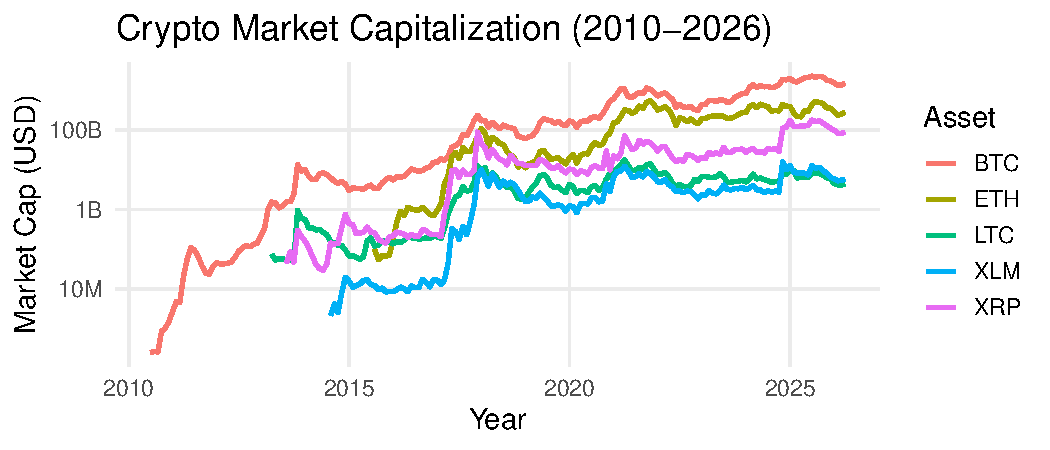
\includegraphics[width=\textwidth]{figures/crypto_plot_final.pdf}
        %\caption{Crypto Market Growth}
 \end{center}       
        %\vspace{0.2cm} % Adds a small gap between plot and text
         \begin{itemize}
         \item Market capitalization of cryptos has reached approximately \$2.57 trillion\footnote{\url{https://coinmarketcap.com/charts/} (Accessed on 18/04/26)}, comparable to the GDP of Italy\footnote{IMF World Economic Outlook, Oct 2025}.
        %\item Italy remains one of the largest economies in Europe.
        \item The general population buys these assets with the hope of making more money.
      \end{itemize}
      \vspace{0.2cm} % Adds a small gap between itemize and footnotes
    \end{frame}

\begin{frame}{A Very Volatile Market}
\begin{center}
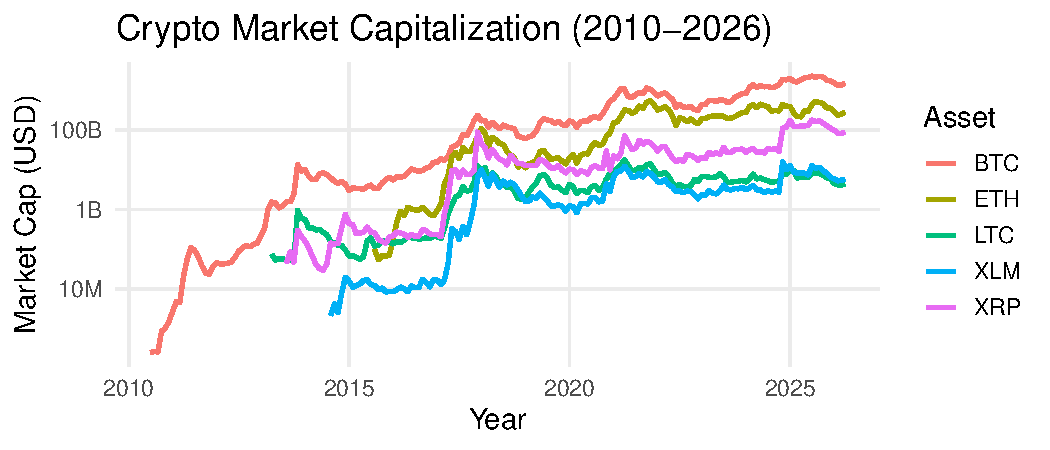
\includegraphics[width=\textwidth]{figures/crypto_plot_final.pdf}
        %\caption{Crypto Market Growth}
 \end{center}       
        %\vspace{0.2cm} % Adds a small gap between plot and text
         \begin{itemize}
         \item  Extreme events happen rather frequently, see figure.
         \item Buying these assets exposes to a risk.
         \item Developing a model to capture the common factors driving these movements. %Quando la presenti metti in evidenza che l'andamento sembra molto simile
         \end{itemize}
     % \vspace{0.2cm} % Adds a small gap between itemize and footnotes
\end{frame}


\section{Factor Model}

\begin{frame}{Dataset Structure}
    \begin{itemize}
        \item \textbf{Dimensions:} $N=5$ assets across $T=1,369$ daily observations.
    \end{itemize}

    \begin{table}[h]
        \centering
        \small
        \begin{tabular}{|l|c|c|c|c|c|}
            \hline
            \textbf{Date (T)}  & \textbf{ETH} &\textbf{BTC}&  \textbf{XRP} & \textbf{LTC}  & \textbf{XLM} \\ \hline
            2016-01-01 & \$0.95 & \$434.33& \$0.006 & \$3.51 & \$0.002 \\ \hline
            \dots & \dots & \dots & \dots & \dots  & \dots \\ \hline
            2019-09-30 & \$179.87 & \$8293.87 & \$0.26 & \$56.06 & \$0.06 \\ \hline
        \end{tabular}
        \caption*{Structure of the $X$ matrix $(T \times N)$.}
    \end{table}

    \begin{itemize}
        \item Only asset prices are present.
        \item Common factors are unobservable.
    \end{itemize}
\end{frame}

\begin{frame}{Factor Model}
    \begin{itemize}
        \item Enables estimation in the presence of \textbf{unobserved predictors}.
        \item Assumes that $X_{i,t}$ is driven by a small, \textbf{unknown number ($k$)} of latent common factors:
    \end{itemize}

    \begin{center}
    \vspace{-0.3cm}
    \begin{equation*}
        X_{i,t} = \phi_i' F_t + u_{i,t}, \quad 
        \begin{cases} 
            i=1,\dots,N \\ 
            t=1,\dots,T 
        \end{cases}
    \end{equation*}
    \end{center}

    \begin{block}{Model Components}
        \begin{description}
            \item[$F_t$] \textbf{Common Factors:}  $k \times 1$ vector of market drivers.
            \item[$\phi_i$] \textbf{Factor Loadings:} $k \times 1$ vector describing the impact of common factors on asset $i$. 
            \item[$u_{i,t}$] \textbf{Idiosyncratic Component:} Residual asset-specific noise.
        \end{description}
    \end{block}
\end{frame}


\begin{frame}{Main Assumptions}
  \begin{itemize}
   \item \textbf{(Weak) Stationarity:} $\mathbb{E}[X_t] = \mu$, $\mathrm{Cov}(X_t,\,X_{t+h}) = \gamma(h)$.
    \item \textbf{Asymptotics:} $\min\{N,T\}\to\infty$.
    \item \textbf{A1 -- Factors:} $\mathbb{E}\lVert F_t\rVert^{4}<\infty$ and
          $\tfrac1T\sum_{t=1}^{T} F_tF_t' \xrightarrow{p} \Sigma_F \succ 0$
          (full rank: identification).
    \item \textbf{A2 -- Loadings (pervasive):}
          $\tfrac1N\sum_{i=1}^{N}\phi_i\phi_i' \to \Sigma_\Phi \succ 0$ ---
          loadings accumulate at rate $N$ (\emph{strong} factors).
    \item \textbf{A3 -- Idiosyncratic (weak dependence):}
          $\mathbb{E}\lvert u_{i,t}\rvert^{8}<\infty$ and, with
          $\mathbb{E}[u_{i,t}u_{j,s}]=\tau_{ij,ts}$, the summability
          $\tfrac1N\sum_{i,j}\lvert\tau_{ij}\rvert<\infty$
          $\Rightarrow \lambda_{\max}(\Sigma_u)=O(1)$.
    \item \textbf{A4 -- Independence:} $\{\phi_i\}$, $\{F_t\}$, $\{u_{i,t}\}$
          are independent groups (hence $\mathbb{E}[u_tF_t']=0$).
  \end{itemize}
\end{frame}

\begin{frame}{Consequence: Eigenvalue Separation}
  We can write the sample covariance $\hat\Sigma_X = \tfrac1T\sum_t X_tX_t'$ as:
  \[
    \hat\Sigma_X =
    \underbrace{\Phi\Big(\tfrac1T\textstyle\sum_t F_tF_t'\Big)\Phi'}_{A}
    \;+\;
    \underbrace{\tfrac1T\big(\Phi F'u + u'F\Phi' + u'u\big)}_{B},
  \]
  with $\Phi = [\phi_1|\dots|\phi_N]'$ the $N\times k$ loading matrix.
  
  By A1--A2, $A$ has $k$ eigenvalues growing at rate $N$ (the other $N{-}k$ are zero);
  by A3--A4, $\lambda_{\max}(B)=o(N)$. Weyl's inequality
  $\lambda_j(A+B)\le \lambda_j(A)+\lambda_{\max}(B)$ then gives
  \[
    \lambda_j(\hat\Sigma_X)\;\ge\; c_0\,N \quad (1\le j\le k),
    \qquad
   \lambda_j(\hat\Sigma_X)\;\le\; c_1\,\tfrac{N}{\sqrt{T}} \quad (j> k).
  \]
  The widening gap is what the information criteria (and PCA) exploit to recover
  the $k$ factors.
\end{frame}
\subsection{Data Exploration}

\begin{frame}{Assumptions Are Satisfied?}
    \begin{center}
        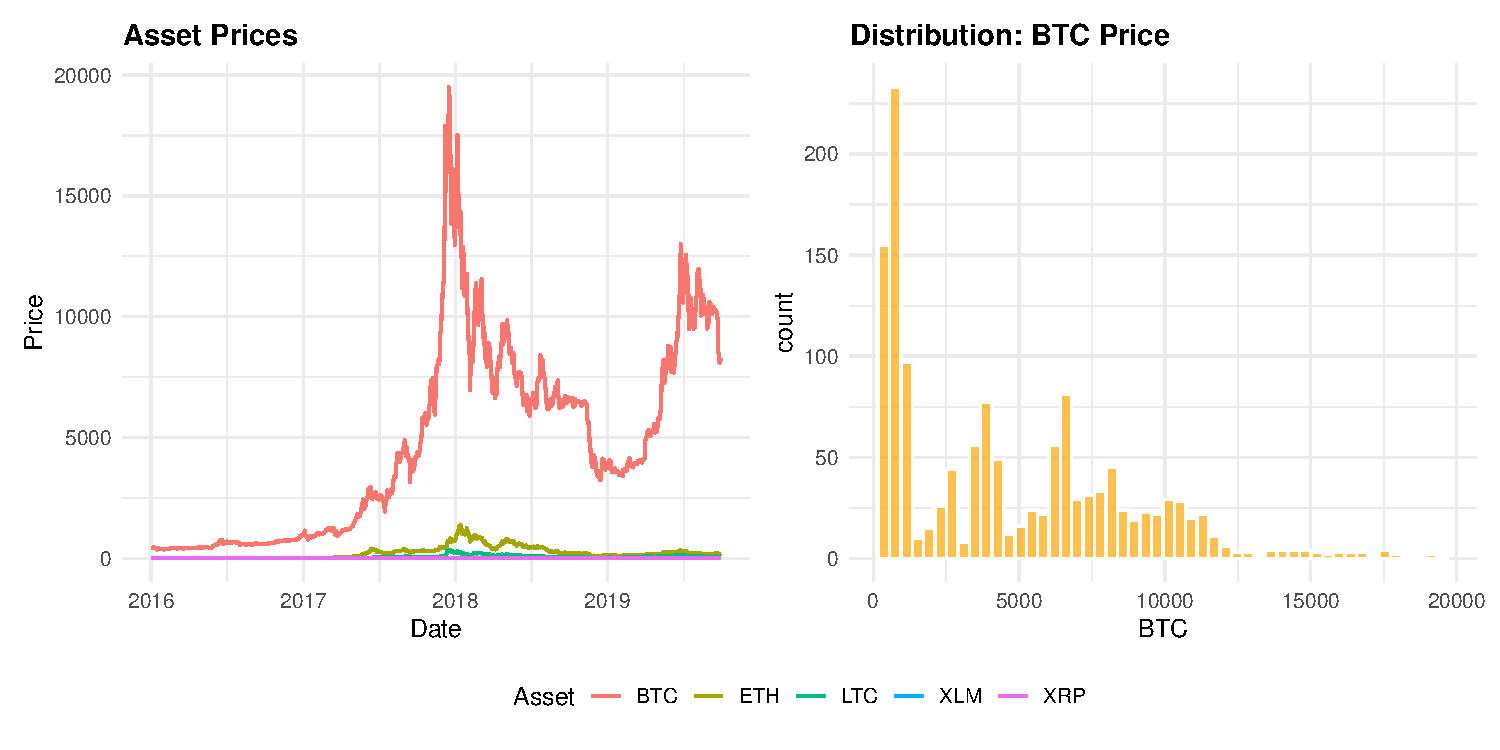
\includegraphics[width=0.9\textwidth]{figures/raw_diagnostics.pdf}
    \end{center}
    \vspace{-0.1cm}
    \begin{itemize}
        \item $N = 5$ is small.
        \item  Prices exhibit a strong upward stochastic trend (non-constant mean).
        \item The BTC histogram shows extreme right-skewness.
        \item  Assets are on different scales.
    \end{itemize}
\end{frame}

\begin{frame}{Data Transformation: Log-Returns}
    \begin{center}
        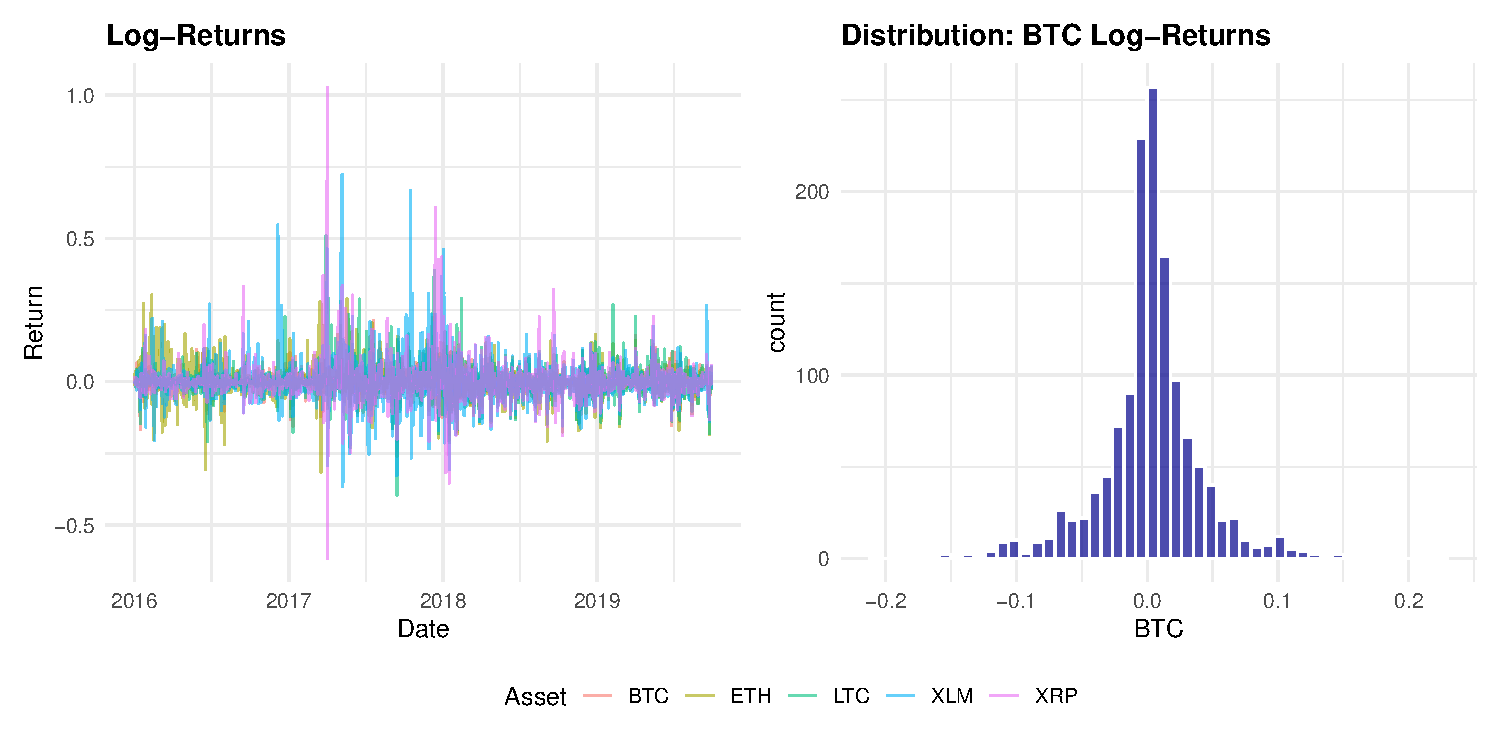
\includegraphics[width=0.9\textwidth]{figures/transformed_diagnostics.pdf}
    \end{center}
    \begin{itemize}
        \item  $y_{i,t} = \ln\left(\frac{x_{i,t}}{x_{i,t-1}}\right) = \ln(x_{i,t}) - \ln(x_{i,t-1})$.
        \item This transformation centers the distribution around zero, stabilizes the variance and reduces the impact of outliers.
         \item  Now assets with vastly different nominal prices are brought to a common scale.
    \end{itemize}
\end{frame}

\subsection{Initial Approach}

\begin{frame}{Initial Approach: Estimating the Number of Common Factors}
    To determine the optimal number of factors $\hat{k}$, we employ the information criteria proposed by \textbf{Bai and Ng (2002)}:
    
    \begin{itemize}
        \item \textbf{Criteria:} We consider $IC_{p1}, IC_{p2},$ and $IC_{p3}$, which balance the minimization of the sum of squared residuals against a penalty for model complexity.
        \item \textbf{Implementation in R:} Utilizing the \texttt{ICr} function from the \textbf{\texttt{dfms}} package, we find $\hat{k}$ such that:
        \begin{equation*}
            \hat{k} = \arg\min_{0 \le k \le k_{max}} IC(k)
        \end{equation*}
        where the search space $k_{max}$ is determined by Schwert’s rule of thumb.
    \end{itemize}
\end{frame}

\begin{frame}{Initial Approach: Static Factor Estimation}
    \begin{itemize}
        \item \textbf{Estimation:} Common factors $\hat{F}_t$ are estimated via Principal Component Analysis (PCA) on the full sample of log-returns.
    \end{itemize}
    \textbf{Limitations:}
    \begin{itemize}
        \item Factors lack direct interpretability.
        \item Difficulty in assessing the model's predictive accuracy.
    \end{itemize}
    \begin{block}{Transition to Stock \& Watson (2002)}
        To evaluate the "goodness of fit," we adopt the \textbf{Stock and Watson methodology}, which enables real-time simulation and benchmarking.
    \end{block}
\end{frame}

\section{Stock \& Watson Methodology}

\begin{frame}{Stock \& Watson Methodology}
    \begin{itemize}
        \item \textbf{Data Split:} The sample is divided into a \textbf{training set} (75\%) and a \textbf{test set} (25\%).
        \item \textbf{Recursive Estimation:} For each time $t$ in the test set:
        \begin{enumerate}
            \item Factors $\hat{F}_t$ are extracted via PCA from the training window.
            \item A linear model is estimated via OLS for each asset using $\hat{F}_t$
            \item A 1-step ahead forecast is generated and stored: $\hat{y}_{i,t+1} = \hat{\beta}'_i \hat{F}_t$.
            \item The training window expands to include the observation at $t$.
        \end{enumerate}
        \item \textbf{Benchmarking:} An \textbf{AR($p$)} model is estimated at each step:
        \begin{equation*}
            y_{i, t+1} = \beta_0 + \sum_{j=1}^{p} \beta_j y_{t-j} + \epsilon_{t+1}
        \end{equation*}
        where $p$ is selected dynamically via \textbf{BIC}.
        \item \textbf{Evaluation:} Model utility is determined by comparing the \textbf{Mean Squared Error (MSE)} of the Factor Model against the AR benchmark.
    \end{itemize}
\end{frame}

\subsection{Main Results}

\begin{frame}{Results: Factor Model vs. AR Benchmark}
    To evaluate performance, we calculate the \textbf{Relative Mean Squared Error} for each asset:
    \begin{equation*}
        \text{RelMSE}_i = \frac{MSE_{i, \text{Factor}}}{MSE_{i, \text{AR}}}
    \end{equation*}
    A ratio $< 1$ indicates that the factor model provides a gain in predictive accuracy over the benchmark.
 \vspace{-0.12cm}
    \textbf{Findings:}
    \vspace{0.12cm}
    \begin{itemize}
        \item For the analyzed cryptocurrencies, the \textbf{Relative MSE is approximately 1} in each case: the factor model and the AR model yield nearly equivalent forecast errors.
        \item For \textbf{3 out of 5 assets} the BIC-optimal lag was \textbf{$p=0$}, while the estimated number of factors saturated its ceiling:
        \begin{equation*}
            \textcolor{red}{\hat{k} = 3 = k_{\max}}.
        \end{equation*}
       It \emph{seems} that A3--A4 are violated , i.e.\ $\lambda_{\max}(B)$ may grow at rate $N$ aswell.
       %\item \textbf{Interpretation:} for the majority of the sample, the best predictor is simply the \textbf{historical sample mean}.%
    \end{itemize}
\end{frame}

\begin{frame}{Robustness Check: Expanding the Cross-Section ($N$)}
    To determine if the previous results were due to the small cross-section ($N=5$), we expanded the dataset using the \textbf{\texttt{crypto2}} package:
    
    \begin{itemize}
        \item We cleaned the data inspired by the methodology of \textbf{Bianchi and Babiak (2021)} to ensure a high-quality data pool.
        \item We increased the number of assets $(N = 29)$ to test if a larger dataset would improve the prediction accuracy.
        \item \textbf{Findings:} 
        \begin{itemize}
            \item The \textbf{Relative MSE results remained analogous} to the small-sample case (RelMSE $\approx$ 1), while the estimated number of factors was $\hat{k} = 1$.
            \item Expanding the number of assets did not yield superior predictive performance over the AR(0) benchmark.
        \end{itemize}
    \end{itemize}

    \begin{block}{The Fundamental Question}
        Does a factor structure actually exist in the data (i.e. $k > 0$)? 
    \end{block}
    \end{frame}
    
   \begin{frame}{Testing for Factor Strength: The Trapani (2018) Test}
    To determine if the factors are "strong" or merely noise, we test the behavior of the eigenvalues $\lambda^{(p)}$ for $p=1, \dots, \hat{k}$ as $N \to \infty$:
    
    \begin{itemize}
        \item \textbf{Hypotheses:}
        \begin{itemize}
            \item $H_0: \lambda^{(p)} = O(N)$ (Diverging eigenvalue; strong factor).
            \item $H_A: \lambda^{(p)} = O(1)$ (Bounded eigenvalue; noise).
        \end{itemize}
        
        \item \textbf{Test Statistic:} Trapani constructs a \textbf{randomized} statistic $\Theta^{(p)}$ that, under $H_0$, follows a chi-squared distribution:
        \begin{equation*}
            \Theta^{(p)} \sim \chi^2(1)
        \end{equation*}
        
        \item \textbf{Decision ($\alpha = 0.01$):} reject $H_0$ when
              $\Theta^{(p)} > \chi^2_{1;\,0.99} \approx 6.63$        
        \item \textbf{Empirical Results:}
        \begin{itemize}
            \item \textbf{Small Dataset ($N=5$):} We reject $H_0$ for the largest eigenvalue ($p=1$). Consequently, $\hat{k}=0$, indicating no evidence of a common factor structure.
            \item \textbf{Expanded Dataset ($N=29$):} We reject $H_0$ for the second largest eigenvalue ($\hat{k}=1$).
        \end{itemize}
    \end{itemize}
\end{frame}    
\begin{frame}{Conclusions}
    This work evaluated the presence and predictive utility of common factors in the cryptocurrency market using the \textbf{Stock \& Watson (2002)} framework and \textbf{Trapani (2018)} test.
    
    \begin{itemize}
        \item \textbf{Predictive Performance:} In both small and large datasets, the factor model yielded a \textbf{Relative MSE $\approx$ 1}, failing to outperform a simple AR(0) benchmark.
        \item \textbf{Identification Sensitivity:} The \textbf{Trapani (2018)} test reveals that factor identification is highly dependent on the cross-sectional dimension ($N$).
        \item \textbf{Sample-Size Dependency:} No consistent factor structure was identifiable for $N=5$ ($\hat{k}=0$), whereas a statistically diverging signal begins to emerge for $N=29$ ($\hat{k}=1$). 
        \end{itemize}
\end{frame}
    
\section*{References}

\begin{frame}[allowframebreaks]{Bibliography}
    \beamertemplatearticlebibitems
    
    \begin{thebibliography}{99}
        
        \bibitem{BaiNg2002}
        J.~Bai and S.~Ng.
        \newblock Determining the Number of Factors in Approximate Factor Models.
        \newblock {\em Econometrica}, 70(1):191--221, 2002.
        
        \bibitem{Bianchi2021}
        D.~Bianchi and M.~Babiak.
        \newblock A factor model for cryptocurrency returns.
        \newblock {\em CERGE-EI Working Paper Series 710}, 2021.
        
        \bibitem{StockWatson2002a}
        J.~H. Stock and M.~W. Watson.
        \newblock Forecasting Using Principal Components From a Large Number of Predictors.
        \newblock {\em Journal of the American Statistical Association}, 97(460):1167--1179, 2002.
        
        \bibitem{StockWatson2002b}
        J.~H. Stock and M.~W. Watson.
        \newblock Macroeconomic Forecasting Using Diffusion Indexes.
        \newblock {\em Journal of Business \& Economic Statistics}, 20(2):147--162, 2002.
        
        \bibitem{Trapani2018}
        L.~Trapani.
        \newblock A Randomized Sequential Procedure to Determine the Number of Factors.
        \newblock {\em Journal of the American Statistical Association}, 113(523):1341--1349, 2018.

    \end{thebibliography}
\end{frame}

\end{document}
%\subsection<presentation>*{For Further Reading}
%
%\begin{frame}[allowframebreaks]
%  \frametitle<presentation>{For Further Reading}
%    
%  \begin{thebibliography}{10}
%    
%  \beamertemplatebookbibitems
%  % Start with overview books.
%
%  \bibitem{Author1990}
%    A.~Author.
%    \newblock {\em Handbook of Everything}.
%    \newblock Some Press, 1990.
% 
%    
%  \beamertemplatearticlebibitems
%  % Followed by interesting articles. Keep the list short. 
%
%  \bibitem{Someone2000}
%    S.~Someone.
%    \newblock On this and that.
%    \newblock {\em Journal of This and That}, 2(1):50--100,
%    2000.
%  \end{thebibliography}
%\end{frame}